% sudah direvisi ibu shofia

\section{Dasar Teori}

\subsection{\textit{Multiple Traveling Salesman Problem}}

Menurut Al-Omeer dan Ahmed, \textit{Multiple Travelling Salesman Problem} (MTSP) adalah salah satu kombinatorial optimasi masalah, yang dapat didefinisikan sebagai berikut: Ada $m$ jumlah salesman yang harus melakukan perjalanan ke $n$ sejumlah kota dimulai dengan depot dan berakhir di depot yang sama \cite{al2019comparative}. Selanjutnya para salesman harus melakukan perjalanan dari satu kota ke kota lain secara terus menerus tanpa mengulang kota mana saja yang telah dilintasi oleh para salesman dan mempertimbangkan jalur terpendek selama perjalanan tersebut. Metode MTSP sebenarnya banyak sekali, namun yang digunakan dalam penelitian ini adalah algoritma genetika dan algoritma \textit{k}-means.

Contoh solusi MTSP:

\begin{figure}[h!]
  \centering
  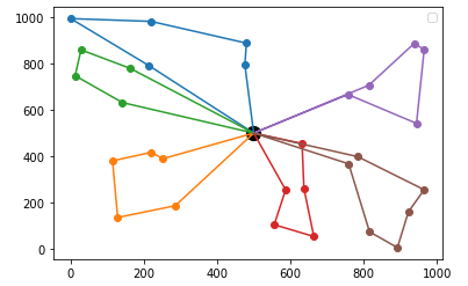
\includegraphics[width=0.5\textwidth]{Picture1.png}
  \caption{Solusi MTSP dengan membagi menjadi 6 klaster}
\end{figure}

\begin{figure}[h!]
  \centering
  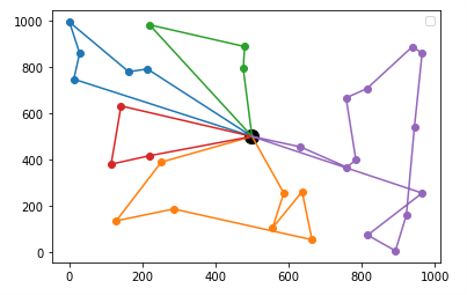
\includegraphics[width=0.5\textwidth]{Picture2.png}
  \caption{Solusi MTSP dengan membagi menjadi 5 klaster}
\end{figure}

\subsection{Algoritma}

Maulana menyebutkan dalam artikelnya algoritma adalah kumpulan perintah untuk menyelesaikan suatu masalah dan diselesaikan dengan cara sistematis, terstruktur dan logis \cite{maulana2017pembelajaran}. Algoritma digunakan untuk memcahkan permasalahan yang dialami oleh seorang pengguna program.

\subsection{Algoritma $k$-means}

$K$-Means adalah jenis metode klasifikasi tanpa pengawasan yang mempartisi item data menjadi satu atau lebih klaster \cite{agusta2007k}. $K$-Means mencoba untuk memodelkan suatu dataset ke dalam klaster-klaster sehingga item-item data dalam suatu klaster memiliki karakteristik yang sama dan memiliki karakteristik yang berbeda dengan cluster lainnya.

Menurut S Monalisa \cite{monalisa2018klasterisasi} tahapan mengklaster menggunakan algoritma \textit{k}-means adalah sebagai berikut:

\begin{enumerate}
	\item Menentukan banyak klaster sesuai dengan keinginan
	\item Pilih beberapa \textit{centroid} secara acak sesuai banyak klaster
	\item Hitung jarak titik ke centroid dengan rumus \textit{euclidean distance}
	\begin{equation}
	d_{xy}=\sqrt{\sum_{i=1}^{n}(x_i-y_i)^{2}}
	\end{equation}
	\item Titik-titik yang tersebar masuk ke klaster yang sama dengan titik \textit{centroid} yang paling dekat
	\item Perbarui \textit{centroid} dengan menghitung nilai rata-rata nilai pada masing-masing klaster
	\item Lakukan iterasi sebanyak mungkin dengan kembali ke tahapan 3 sampai tidak ada perubahan klaster atau perubahan nilai \textit{centroid}
\end{enumerate}

\subsection{Algoritma Genetika}

Pada artikel Hermanto disebutkan bahwa algoritma genetika adalah algoritma yang digunakan untuk mencari solusi suatu permasalahan dengan cara yang lebih alami yang terispirasi dari teori evolusi  \cite{hermawanto2003algoritma}. Dalam hal ini, algoritma genetika dapat juga digunakan untuk pencarian sebuah rute terpendek dalam sebuah kasus perjalanan.

Menurut Armanda RS \cite{armanda2016penerapan} dalam artikelnya menyampaikan penyelesaian masalah menggunakan algoritma genetika memerlukan beberapa tahapan sebagai berikut:

\begin{enumerate}
	\item Menyiapkan populasi, dalam penelitian ini yang digunakan adalah data yang telah diklaster menggunakan algoritma \textit{k}-means
	\item Melakukan reproduksi dengan crosover dan mutasi pada pembentukan awal populasi
	\item Seleksi dengan metode elitism
	\item Menentukan nilai fitness agar mendapatkan solusi akhir yang optimal. Berikut merupakan persamaan perhitungan dalam mengetahui nilai fitness pada metode algoritma genetika
	\begin{equation}
	fitness=\frac{10000}{RMSE}
	\end{equation}
	\item Iterasi dilakukan untuk generasi berikutnya.
\end{enumerate}